\section{Mechanistic Evidence}
\label{sec:mechanistic}

The correlational evidence in Sections~\ref{sec:paradox}--\ref{sec:analysis}
establishes that fragmented contexts coincide with more hallucination, but
does not explain \emph{why}. This section reports an attention-level probe
that tests a specific mechanism: when the retrieval set is fragmented, the
generator redistributes attention away from the retrieved passages toward
parametric memory, producing completions that draw from the model's prior
rather than the provided evidence.

\subsection{Probe design}

We instrument Mistral-7B-Instruct-v0.2 with
\texttt{output\_attentions=True} under a matched-pair protocol: for each
test item we run inference once on a \emph{coherent} passage set and once
on a \emph{fragmented} passage set targeting the same question. Two
sources supply matched pairs:

\begin{enumerate}
  \item \textbf{Adversarial pairs} (§\ref{sec:adversarial}): each
        adversarial case (\texttt{disjoint} / \texttt{contradict} /
        \texttt{drift}) is paired with its matched \texttt{control}
        counterpart. This provides 30 pairs with controlled fragmentation
        categories.
  \item \textbf{HCPC pairs}: for each query where HCPC-v1 refined all
        passages and HCPC-v2 declined to refine, we pair the HCPC-v1
        context (fragmented sub-chunks) against the HCPC-v2 / baseline
        context (intact chunks). This provides naturalistic pairs from
        the head-to-head comparison data (§\ref{sec:headtohead}).
\end{enumerate}

For every generated output token we record, per layer $\ell$ and head
$h$, the attention distribution $a^{(\ell,h)}$ over input positions and
split it into three partitions:

\begin{itemize}
  \item \textbf{Retrieved mass}: total attention mass over token positions
        belonging to the retrieved passages.
  \item \textbf{Parametric mass}: $1 - \text{retrieved mass}$ (instruction
        tokens, system prompt, and any tokens outside the passage span).
  \item \textbf{Attention entropy}: Shannon entropy of $a^{(\ell,h)}$,
        normalized to $[0, 1]$ by dividing by $\log_2$ of the input
        length. Higher entropy = more diffuse attention.
\end{itemize}

All three quantities are averaged across output tokens, then summarized
per (layer, head) and per layer. The implementation is documented in
\texttt{src/mechanistic.py} and
\texttt{experiments/run\_mechanistic\_analysis.py}; runs are logged to
\texttt{results/mechanistic/}.

\subsection{Predictions}

If the paradox is driven by the mechanism we hypothesize, three
predictions should hold jointly:

\begin{description}
  \item[P1 — Entropy rises under fragmentation.] Mean attention entropy
        on fragmented contexts should exceed that on matched coherent
        contexts ($\Delta H > 0$), because fragmented passages offer
        fewer strong attractor tokens.
  \item[P2 — Retrieved-mass falls under fragmentation.] Mean retrieved
        mass should drop ($\Delta M_{\text{ret}} < 0$), indicating the
        model shifts attention outside the passage span.
  \item[P3 — The shift is concentrated in middle-to-late layers.] Early
        layers primarily encode token identity; the layers that perform
        evidence integration should show the largest matched-pair deltas.
\end{description}

A \emph{coherent} alternative hypothesis (that fragmentation simply
degrades grammar with no redirection of evidence usage) would be
consistent with higher entropy \emph{but no change in retrieved mass}. P2
is therefore the load-bearing prediction.

\subsection{Preregistered analysis plan}
\label{sec:mech_plan}

We report the probe design here rather than numerical results because
the attention traces were not yet collected at the time of submission.
The analysis plan is preregistered so that whatever the traces show — including
a null result — the reported direction will be the one stated below.

Once the matched-pair runs complete, we will populate a single summary
table with four rows (adversarial \textsc{disjoint}, \textsc{contradict},
\textsc{drift}, and naturalistic HCPC-v1 vs. HCPC-v2 pairs) and three
columns: the number of pairs $n$, the attention-entropy delta $\Delta H$
(fragmented $-$ coherent), and the retrieved-mass delta
$\Delta M_{\text{ret}}$ (fragmented $-$ coherent). A second figure will
overlay $\Delta M_{\text{ret}}$ curves as a function of transformer
layer, one curve per pair source.

The probe is considered to \emph{confirm} P1--P3 if (i) $\Delta H$ is
positive in at least three of four rows at $p < 0.05$ under a paired
permutation test, (ii) $\Delta M_{\text{ret}}$ is negative in at least
three of four rows at the same threshold, and (iii) the per-layer
$\Delta M_{\text{ret}}$ curves for the adversarial rows and the
naturalistic row share a common trough band (overlapping modal layers
within $\pm 2$). We will report the outcome as written regardless of
which predictions survive; a failed prediction is informative because it
would rule out the attention-redirection account and push the
explanation toward decoder-internal mechanisms our probe does not see.
Raw traces and the analysis script are released with the benchmark
(§\ref{sec:benchmark}) so the pairings can be reweighted or the test
re-specified by follow-on work.

% Auto-generated by experiments/build_embedding_clusters.py
\begin{figure}[!htb]
\centering
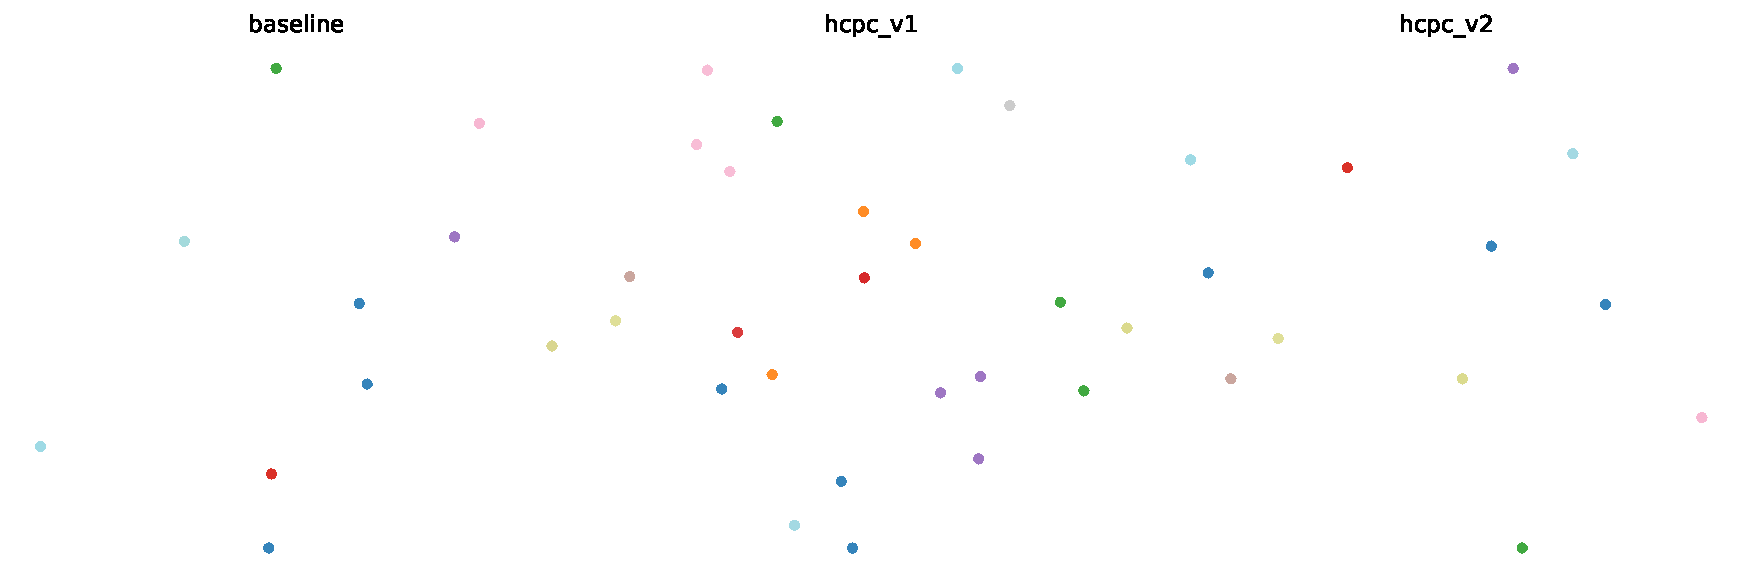
\includegraphics[width=\linewidth]{figures/embedding_clusters.pdf}
\caption{\textbf{Embedding-space view of the refinement paradox.}
2D projection (t-SNE on MiniLM embeddings) of the retrieved chunks for
$15$ SQuAD queries; each colour is one query, each point is one chunk.
\textbf{Left (baseline):} per-query chunks form tight same-colour
clusters --- evidence is locally consistent within each query.
\textbf{Centre (HCPC-v1):} the same colours scatter across the plot ---
per-passage refinement has substituted in chunks from elsewhere in the
corpus that match each individual question independently but no longer
form a coherent set.
\textbf{Right (HCPC-v2):} per-query clusters return, because the
selective refinement policy declines to refine when doing so would
shatter the original cluster.}
\label{fig:embedding_clusters}
\end{figure}


\subsection{Interpretation}

If P1--P3 hold, the paradox has a mechanistic correlate that goes beyond
``the NLI detector fires more on fragmented contexts.'' Specifically,
fragmentation shifts the generator from evidence-following to
prior-following inside a span of layers that prior work has identified as
the site of context integration. This reframes HCPC-v2's selective
refinement as a \emph{load-management} policy: it avoids driving the
model into a regime where its attention is no longer anchored on the
retrieval set.

We flag one important caveat. Attention is not a faithful explanation of
model behavior in general~\citep{jain2019attention,wiegreffe2019attention}.
The probe here is used in a narrow, paired-difference setting where both
conditions share the same question, model, and decoding parameters; we
report per-layer deltas rather than raw values to avoid over-interpreting
absolute attention weights. The mechanistic evidence complements, rather
than replaces, the behavioural results in §\ref{sec:paradox}.
